%%%%%%%%%%%%%%%%%%%%%%%%%%%%%%%%%%%%%%%%%%%%%%%%%%%%%%%%%%%%%%%%%%%%%%%%%%%%%%%%%%%%%%%%%%
\section{Evaluation}
%%%%%%%%%%%%%%%%%%%%%%%%%%%%%%%%%%%%%%%%%%%%%%%%%%%%%%%%%%%%%%%%%%%%%%%%%%%%%%%%%%%%%%%%%%i
\subsection{Security: do we meet our meet security goals}
   - attack scenarios

\subsection{Performance}

We measure two aspects of \sys's performance: (1) the latency and storage cost of using \sys's
low-level API to apply a disguise, reveal a disguise, or temporarily recorrelate disguised data; and
(2) the impact of these disguising operations on the performance of concurrently executing
application users.

We evaluate performance using three applications: WebSubmit-rs, HotCRP, and Lobsters.

WebSubmit is an answers-submission application for course lectures (similar to \lyt{TODO other
course submission apps}). Its simple schema consists of lectures, questions, answers, and user
accounts; each user owns their account and a set of answers. We integrated \sys into WebSubmit to
support a disguise for admin-anonymization of all answers; a disguise for per-user GDPR-compliant
account deletion; account restoration after deletion; and answer editing after anonymization.
\sys-WebSubmit is a fully-E2E application that supports additional endpoints to perform these
disguise actions, and emails users their capabilities and locators (as these endpoints) when
disguise actions are performed.

\lyt{TODO describe HotCRP and Lobsters.}

\head{Latency Costs of Disguise-Related Actions.}
\begin{table}[t!]
\begin{center}
\begin{tabular}{ c c }
    \textbf{High-Level Op (20 Lectures, 4 Answers/Lecture)} & \textbf{Time (mus)}\\
\hline
    Create User Account & 1000\\
    Anonymize User Account & 18500\\
    Edit Normal Lecture Answer & 2000 \\
    Edit Anonymized Lecture Answer & 62000 \\
    Delete User Account (Pre-Anon) & 25000 \\
    Delete User Account (Post-Anon) & 105000 \\
    Restore User Account & 366000 \\
\hline
    \textbf{DB Op} & \textbf{Time (mus)}\\
\hline
Insert DB Row (User )& 120\\
Update DB Row (FK) & 64\\ 
Select DB Row (User) & 120\\
Remove DB Row (User) & 90\\
Select DB Rows (Answers) & 160\\
Remove DB Rows (Answers) & 150\\
Reveal Deleted Row (DB Select + Insert) & 160 \\
Create + Register Principal & 110\\
\hline
    \textbf{Crypto Op} & \textbf{Time (mus)}\\
\hline
Generate Keypair & 300831\\
Encrypt Ownership Token & 360\\
Decrypt Ownership Token & 3000\\
Encrypt Diff Token & 340\\
Decrypt Diff Token & 3000\\
\end{tabular}
\end{center}
\caption{Amount of time required to run different operations for disguises in WebSubmit.}
    \label{tab:opstats}
\end{table}

Table~\ref{tab:opstats} shows the latency of different WebSubmit disguise-related operations. 
The latency of each high-level operation shown scales linearly with the amount
of data (\ie number of answers) associated with each user. Each high-level operation requires some number of DB or crypto operations.

Creating an account in WebSubmit generates an APIKey and registers a private-public keypair for the
user (emailing the user the public key as the user's decryption capability).

Account anonymization generates one pseudoprincipal per lecture, so that all of a user's answers for
a particular lecture belong to the same pseudoprincipal.
Anonymization selects the relevant answers to anonymize; generates per-lecture
pseudoprincipals and ownership tokens; encrypts and stores these ownership tokens; and
performs DB
queries to insert pseudoprincipls and to update answer FKs to point to these new pseudopricipals.

Editing answers normally simply performs update DB queries. Editing anonymized answers, however,
uses client-provided locator and decryption capabilities to authorize the client to speak for the
pseudoprincipal associated with the answer.  \sys performs this authorization check by decrypting
\emph{all} ownership tokens at the specified locator until it finds a ownership token linking the
client to the currently-owning pseudoprincipal. For example, this benchmark's anonymization of a
user account generates 20 ownership token ciphertexts at the same locator; editing anonymized
answers of a single lecture thus performs up to 20 decryptions to determine which pseudoprincipals
the client can act for. This can be optimized by batching all ownership tokens from one disguise
into a single encrypted ciphertext.

Account deletion pre-anonymization does not perform any composition using accessible
ownership; \sys simply selects answers of the user to remove; removes these answers; and encrypts
and inserts one diff token for each answer.

Account deletion post-anonymization first uses a decryption capability and locator to find and decrypt
ownership tokens of the user. This lets \sys find data of pseudoprincipals that the user is authorized to
remove along with their account, and compose account deletion on top of anonymizaton.
\sys decrypts one ownership token for each lecture; selects answers of both
the user and any linked pseudoprincipals to remove; and like before, removes these answers and
encrypts and inserts one diff token for each answer.

Account restoration decrypts a diff token for each answer for each lecture, and performs DB checks
to ensure the diffs can be restored (\eg that the corresponding lecture of an answer to reinsert
still exists). If the checks pass (which they do in this benchmark), restoration reinserts the
answers stored in the diffs.

\head{Storage Costs of Disguise-Related Actions.}
Each generated pseudoprincipal adds an additional row to the users table in WebSubmit; \sys also stores public-key metadata for each principal (and
pseudoprincipal), and (in-memory) encrypted ciphertexts for tokens.
Clients keep track of capabilities and locators that are emailed to them in the form of URLs that
allow for account restoration or post-anonymization answer editing.

\head{Impact on Normal Application Execution.}

\subsection{Case studies}
   1) websubmit
      - was Edna sufficient for the application's needs?
      - changes to application required (how much work to integrate Edna?)
      - *how* did application use Edna?
        - what disguises?
        - how caps integrated with application?
   2) HotCRP
   3) Lobsters?

\begin{figure*}[t!]
    \centering
    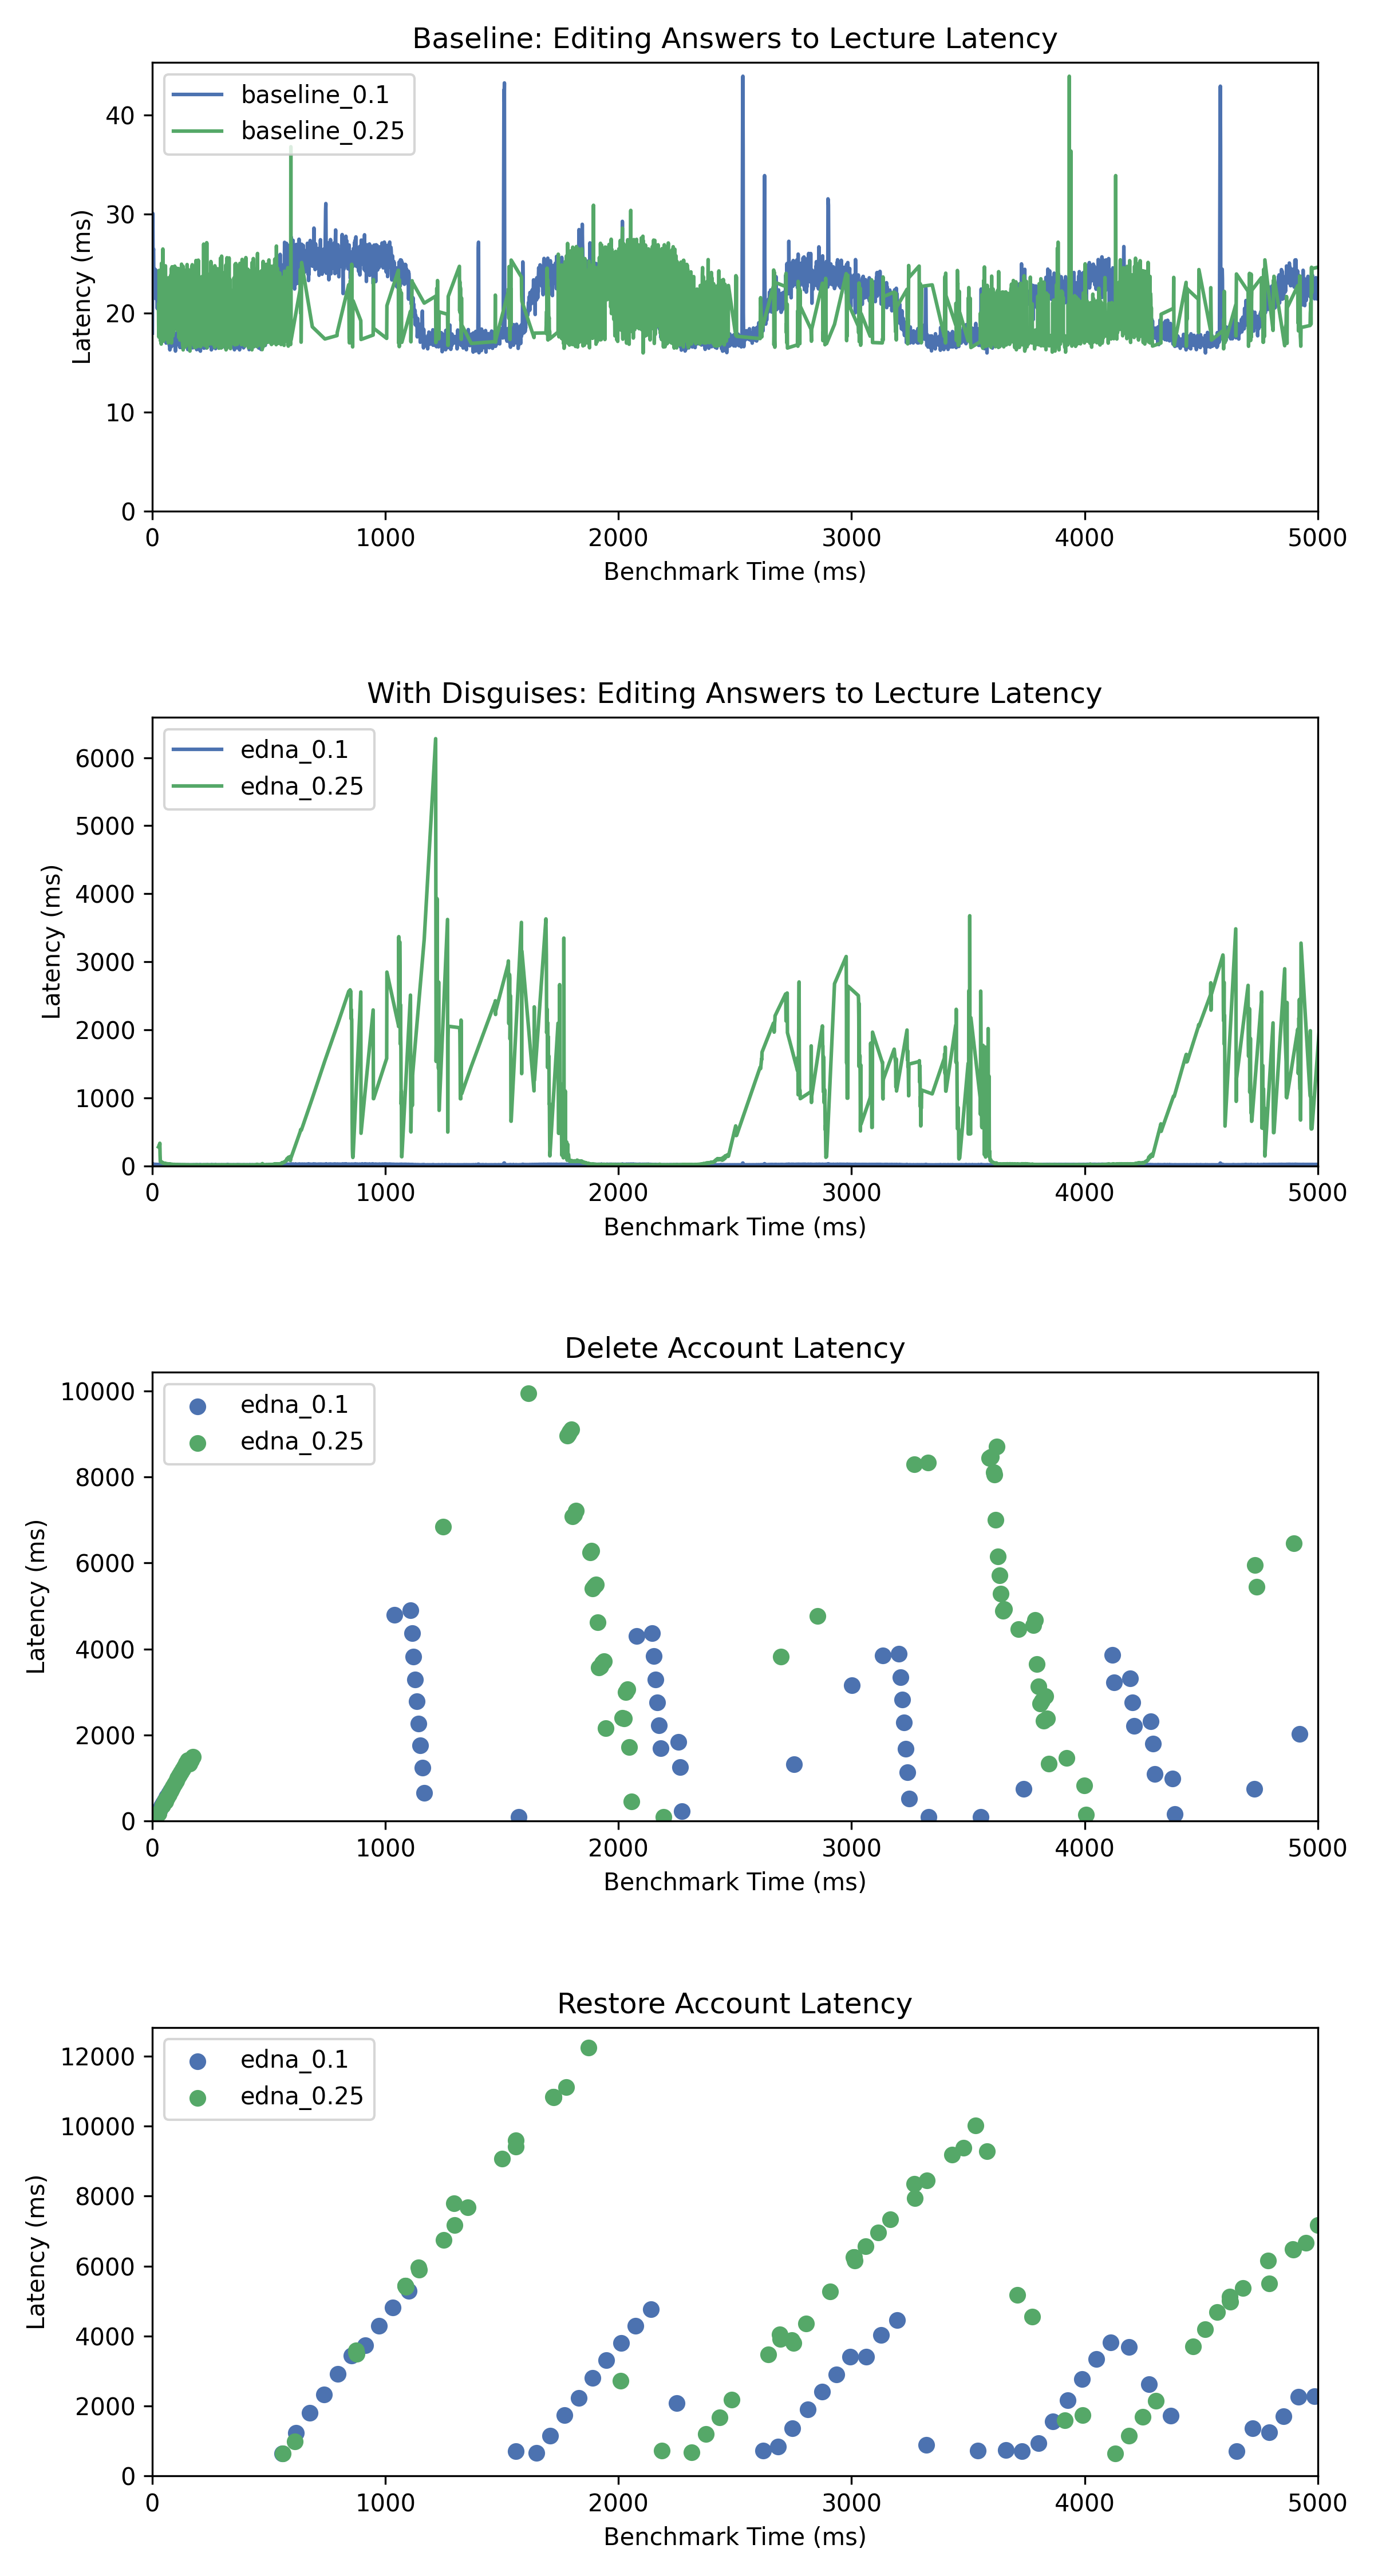
\includegraphics[width=0.45\textwidth]{figs/concurrent_results_40lec_100users}
    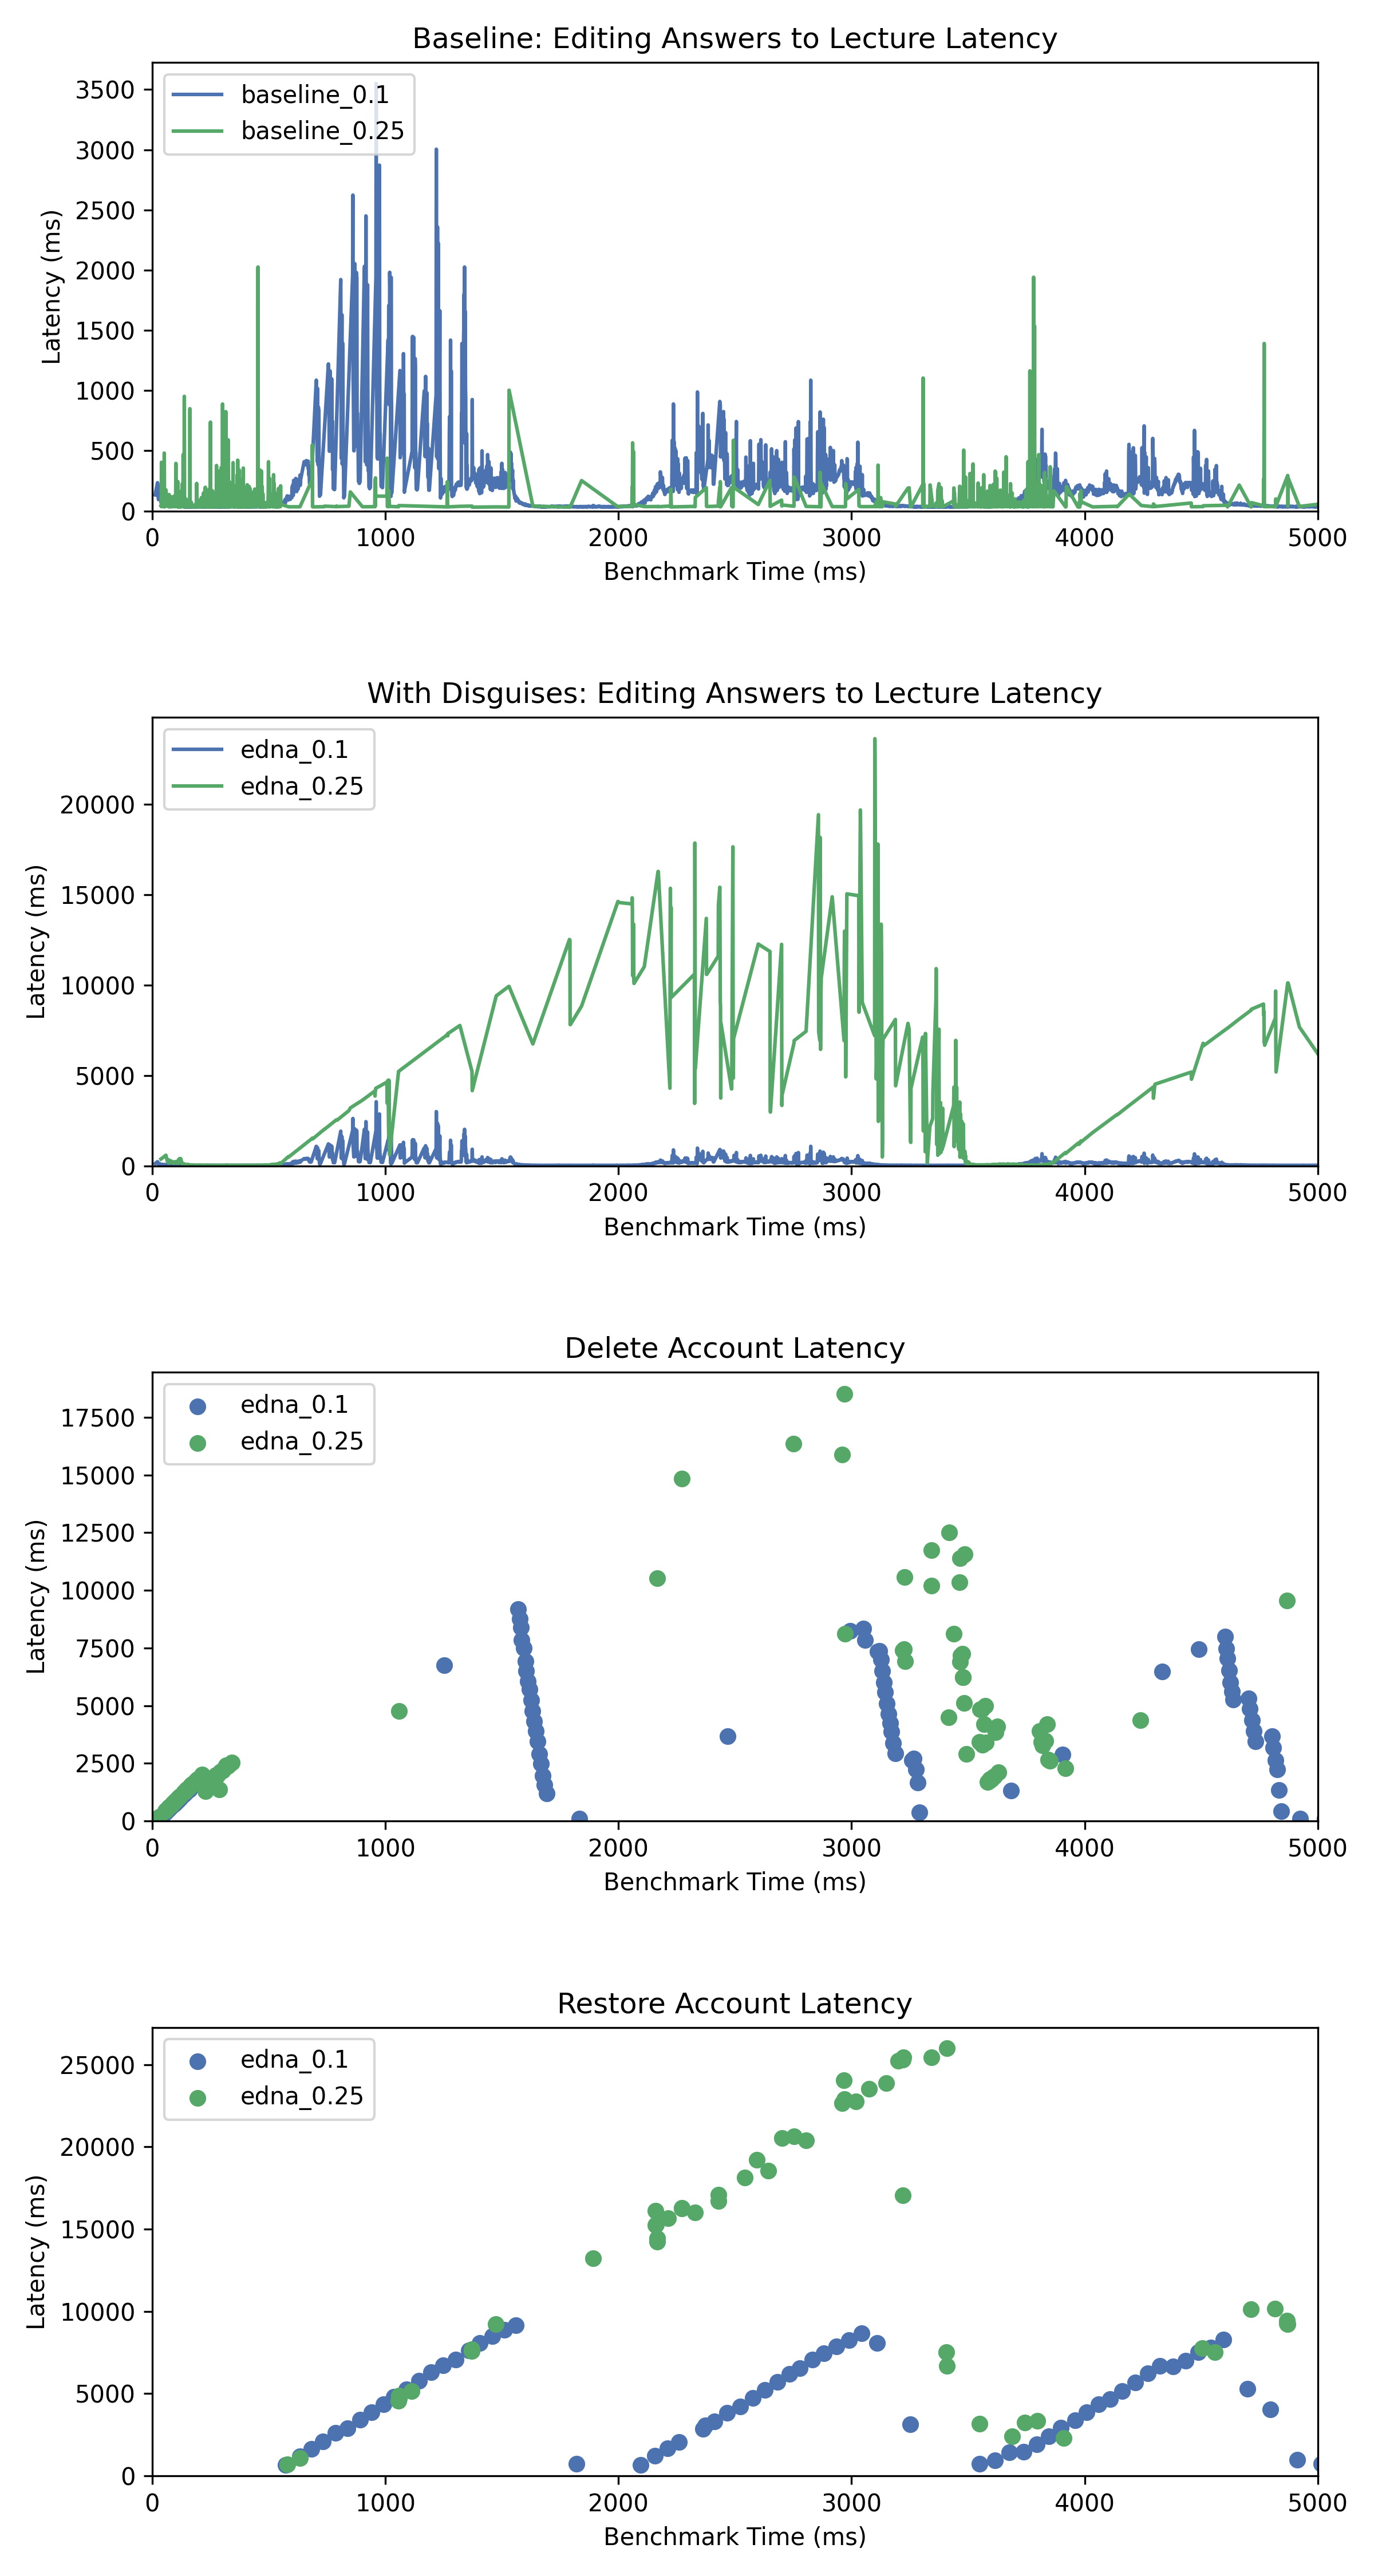
\includegraphics[width=0.45\textwidth]{figs/concurrent_results_40lec_200users}
    \caption{100 Users (left), 200 users (right); 
    40 lectures; 4 questions/lecture; ~5s sleep between disguise and reveal. }
\end{figure*}


